\section{Boltzmann Machine}
In this thesis we are going to use a slightly different type of neural network, called a Boltzmann machine. First major contribution to Boltzmann machines comes from G. E Hinton and T.J. Sejnowski in 1983 \cite{ancoopcomp}. The neural net is a generative model which learns by matching the probability distribution of its inputs. 

\subsection{Structure and training}

A Boltzmann machine has interconnected nodes within a layer.

\begin{figure}[H]
    \centering
    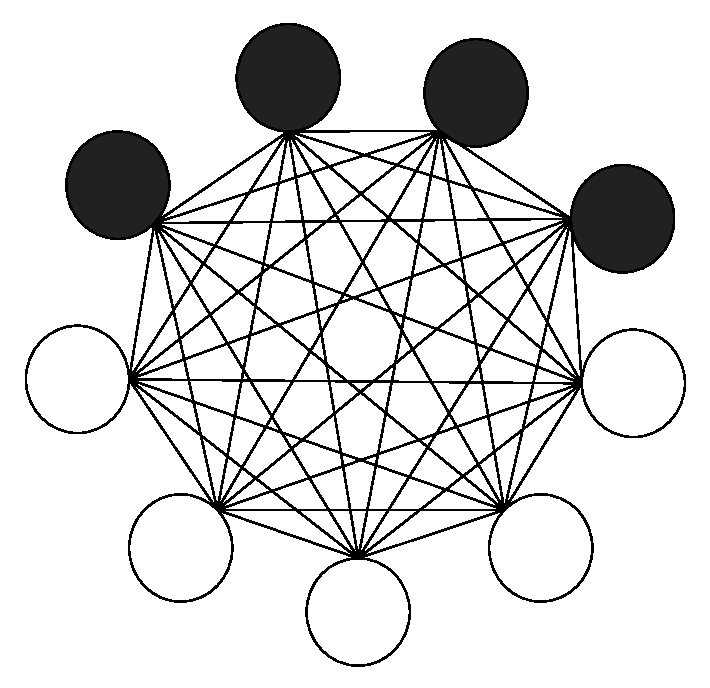
\includegraphics[width=0.7\textwidth]{Figures/Drawn/machinelearning/boltzmann1.pdf}
    \caption{A unrestricted Boltzmann machine where every node is connected. Here the black nodes are the visible layer while the white nodes constitute the hidden layer. }
    \label{fig:boltz1}
\end{figure}

The nodes are binary, being able to take the value $0$ or $1$, have a weights $w_{ij}$ for connection strength between node $v_i$ and $h_j$ and biases $a_i$ for the visible layer and $b_j$ for the hidden layer. For a system of $N_h$ hidden neurons and $N_v$ visible neurons we have the probability distribution of nodes taking the value $1$ defined as

\begin{equation}
    P(\boldsymbol{v},\boldsymbol{h}) = \frac{1}{Z} e^{-E(\boldsymbol{v},\boldsymbol{h})} \; ,
\end{equation}

where the energy of the model is given by

\begin{equation}
    E(\boldsymbol{v},\boldsymbol{h}) = -\sum_i^{N_v} a_i v_i - \sum_j^{N_h} b_j h_j -\sum_i^{N_v} \sum_j^{N_h} v_i w_{ij} h_j
\end{equation}

and the normalization factor

\begin{equation}
    Z = \sum_{ \boldsymbol{v}, \boldsymbol{h}} e^{-E(\boldsymbol{v},\boldsymbol{h})} \; ,
\end{equation}

where we sum over all possible states of the model, which increases exponentially as $2^{(N_v + N_h)}$. The marginal distribution over the visual layer can be written as

\begin{equation}
    P(\boldsymbol{v}) = \sum_{\boldsymbol{h}} \frac{1}{Z} e^{-E(\boldsymbol{v}, \boldsymbol{h})}
\end{equation}

To train a Boltzmann machine we need to have a cost function that compares the predicted distribution of the model and the actual distribution of the data set. As such we will use the Kullback-Leibler divergence as a cost function:

\begin{equation}
    KL(\boldsymbol{W}, \boldsymbol{a}, \boldsymbol{b}) = \sum_{(\boldsymbol{v}, \boldsymbol{h})} R(\boldsymbol{v}) \log{\frac{R(\boldsymbol{v})}{P(\boldsymbol{v})}} \; ,
\end{equation}

where $R(\boldsymbol{v})$ is the distribution we want to approximate and $P(\boldsymbol{v})$ is the distribution of the neural network model. Following the derivations of A.L. Yuille \cite{boltzderv} we have that

\begin{equation}\label{eq:costderv}
    \frac{ \partial KL(\boldsymbol{W}, \boldsymbol{a}, \boldsymbol{b})}{\partial w_{ij}} = - \sum_{(\boldsymbol{v}, \boldsymbol{h})} \frac{ R(\boldsymbol{v})}{P( \boldsymbol{v})} \frac{\partial P( \boldsymbol{v})}{\partial w_{ij}} \; ,
\end{equation}

where we further have

\begin{equation}
    \frac{\partial P(\boldsymbol{v})}{\partial w_{ij}} = \frac{1}{Z} \frac{\partial}{\partial w_{ij}} \sum_{\boldsymbol{h}} e^{-E(\boldsymbol{v}, \boldsymbol{h})} - \frac{1}{Z}  \sum_{\boldsymbol{h}} e^{-E(\boldsymbol{v}, \boldsymbol{h})} \frac{\partial \log{Z} }{\partial w_{ij}}
\end{equation}

which we can express as

\begin{equation}
    \frac{\partial P(\boldsymbol{v})}{\partial w_{ij}} = - \sum_{\boldsymbol{h}} v_i h_j P(\boldsymbol{v},\boldsymbol{h}) + \sum_{\boldsymbol{h}} \left [ P(\boldsymbol{v},\boldsymbol{h}) \sum_{\boldsymbol{v},\boldsymbol{h}} v_i h_j P(\boldsymbol{v},\boldsymbol{h})  \right ] \; .
\end{equation}

Then
\begin{equation} \label{eq:modelderv}
     \frac{\partial P(\boldsymbol{v})}{\partial w_{ij}} = - \sum_{\boldsymbol{h}} v_i h_j P(\boldsymbol{v},\boldsymbol{h}) + P(\boldsymbol{v},\boldsymbol{h}) \sum_{\boldsymbol{v},\boldsymbol{h}} v_i h_j P(\boldsymbol{v},\boldsymbol{h}) \; .
\end{equation}

Using the result of equation \ref{eq:modelderv} in equation \ref{eq:costderv} we get that

\begin{equation}
    \frac{ \partial KL(\boldsymbol{W}, \boldsymbol{a}, \boldsymbol{b})}{\partial w_{ij}} = \sum_{\boldsymbol{v},\boldsymbol{h}} v_i h_j \frac{P(\boldsymbol{v},\boldsymbol{h})}{P(\boldsymbol{v})} R(\boldsymbol{v}) - \left [\sum_{\boldsymbol{v},\boldsymbol{h}} R(\boldsymbol{v})\right ] \sum_{\boldsymbol{v},\boldsymbol{h}} v_i h_j P(\boldsymbol{v},\boldsymbol{h}) \; ,
\end{equation}

which we can simplify

\begin{equation}
    \frac{ \partial KL(\boldsymbol{W}, \boldsymbol{a}, \boldsymbol{b})}{\partial w_{ij}} = \sum_{\boldsymbol{v},\boldsymbol{h}} v_i h_j P(\boldsymbol{h} | \boldsymbol{v}) R(\boldsymbol{v}) - \sum_{\boldsymbol{v},\boldsymbol{h}} v_i h_j P(\boldsymbol{v},\boldsymbol{h}) \; ,
\end{equation}

where we require that

\begin{equation}
     \frac{\partial \log{Z} }{\partial w_{ij}} = \sum_{\boldsymbol{v},\boldsymbol{h}} v_i h_j P(\boldsymbol{v},\boldsymbol{h}) \; .
\end{equation}
We then define the expectation, or correlation, values

\begin{equation}
    \left < v_i h_j \right >_{\text{data}} = P(\boldsymbol{h} | \boldsymbol{v}) R(\boldsymbol{v})
\end{equation}

and

\begin{equation}
    \left < v_i h_j \right >_{\text{model}} = P(\boldsymbol{v}, \boldsymbol{h}) \; .
\end{equation}

This gives us the update rule

\begin{equation}\label{eq:wdiff}
    \Delta w_{ij} = - \eta \left ( \left < v_i h_j \right >_{\text{data}} - \left < v_i h_j \right >_{\text{model}} \right ) \; . 
\end{equation}
\subsection{Restricted Boltzmann machine}
Estimating $ \left < v_i h_j \right >_{\text{data}}$ and $ \left < v_i h_j \right >$ is done by Gibbs sampling, which is explained in a later chapter, but can be inefficient and take a long time to converge for complex models. Removing the weights between nodes within the same layer we can alleviate much of the computational cost of training. This type of Boltzmann machine is called a restricted Boltzmann machine, or RBM:

\begin{figure}[H]
    \centering
    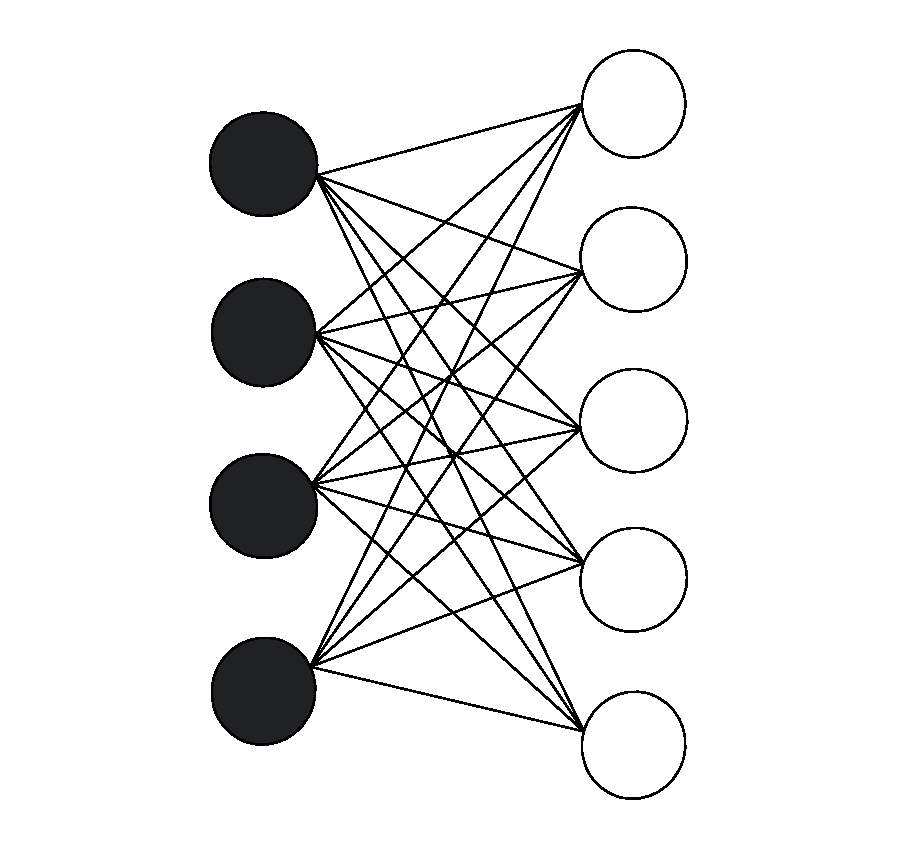
\includegraphics[width=0.7\textwidth]{Figures/Drawn/machinelearning/boltzrest.pdf}
    \caption{A restricted Boltzmann machine where there are no connections between nodes within the same layer. The white nodes are hidden while the black ones are the visible nodes.}
    \label{fig:boltzrest}
\end{figure}

Making the nodes independent of nodes in the same layer means we can write the conditional distributions as

\begin{equation}
    P(\boldsymbol{v} | \boldsymbol{h} ) = \prod_{i \in \boldsymbol{v}} P(v_i | \boldsymbol{h} ) \; , 
\end{equation}

and
\begin{equation}
    P(\boldsymbol{h} | \boldsymbol{v} ) = \prod_{j \in \boldsymbol{h}} P(h_j | \boldsymbol{v} ) \; .
\end{equation}

In a RBM we first have a forward pass where we insert the input data into the visual layer, then we sample the hidden layer by the distribution:

\begin{equation}
    p(h_j^{(0)} = 1 | \boldsymbol{z}_{v}^{(0)}) = \sigma\left (\boldsymbol{z}_{v}^{(0)} \otimes \boldsymbol{W} + \boldsymbol{b} \right ) \; , 
\end{equation}

where our activation function $\sigma$ is the Sigmoid function \ref{Tab:sigmoid}. The index $(0)$ indicate that it is the first pass-through the neural network. As the nodes are binary we then take a sample from $p(h_j^{(0)}=1 | \boldsymbol{z}_v^{(0)} )$ as a Bernoulli distribution, which means each $z_{h, j}^{(0)}$ takes the value $1$ with probability $h_j^{(0)}$. After the forward pass we have a backward pass where we sample from the hidden layer

\begin{equation}
    p(v_j^{(1)} = 1 | \boldsymbol{z}_{h}^{(0)}) = \sigma\left (\boldsymbol{z}_{h}^{(0)} \otimes \boldsymbol{W} + \boldsymbol{a} \right ) \; , 
\end{equation}

where we then convert it to binary values as well. For a continuous valued output it is optional to let the last visual output to remain as a probability distribution. Estimating $\left < v_i h_j \right >_{\text{data}}$ is done by sampling from $P(\boldsymbol{h} | \boldsymbol{v} )$

\begin{equation}
    \left < \boldsymbol{v} \boldsymbol{h} \right >_{\text{data}} = \boldsymbol{z}_v^{(0)} \otimes p(\boldsymbol{h}^{(0)} | \boldsymbol{z}_{v}^{(0)})
\end{equation} \; ,

while estimating $ \left < v_i h_j \right >_{\text{model}}$ requires that we let the model sufficiently affect the output. To do this we do Gibbs sampling through $k$ iterations of the forward and backward passes. Then we have

\begin{equation}
    \left < \boldsymbol{v} \boldsymbol{h} \right >_{\text{model}} = \boldsymbol{z}_v^{(k)} \otimes p(\boldsymbol{h}^{(k)} | \boldsymbol{z}_{v}^{(k)})
\end{equation} \; .

And from \ref{eq:wdiff} the change in weight becomes

\begin{equation}
    \Delta \boldsymbol{W} = \boldsymbol{z}_v^{(0)} \otimes p(\boldsymbol{h}^{(0)} | \boldsymbol{z}_{v}^{(0)}) - \boldsymbol{z}_v^{(k)} \otimes p(\boldsymbol{h}^{(k)} | \boldsymbol{z}_{v}^{(k)}) \; .
\end{equation}
